\title{2016 年高考数学 全国II卷-文科}
\date{}
\maketitle

\section*{一、选择题}
本大题共12小题，每小题5分，在每小题给出四个选项，只有一个选项符合题目要求。

\begin{question}[points=5]
已知集合$A=\{1,2,3\}$，$B=\{x|x^2<9\}$，则$A\cap B=$
\begin{choices}
  \item $\{-2,-1,0,1,2,3\}$
  \item $\{-2,-1,0,1,2\}$
  \item $\{1,2,3\}$
  \item $\{1,2\}$
\end{choices}
\begin{solution}
\textbf{答案：}$\{1,2\}$

\textbf{分析：}由$B=\{x|x^2<9\}=\{x|-3<x<3\}$，所以$A\cap B=\{1,2\}$。
\end{solution}
\end{question}

\begin{question}[points=5]
设复数$z$满足$z+i=3-i$，则$\overline{z}=$
\begin{choices}
  \item $-1+2i$
  \item $1-2i$
  \item $3+2i$
  \item $3-2i$
\end{choices}
\begin{solution}
\textbf{答案：}$3+2i$

\textbf{分析：}由$z+i=3-i$得$z=3-2i$，所以$\overline{z}=3+2i$。
\end{solution}
\end{question}

\begin{question}[points=5]
函数$y=A\sin(\omega x+\varphi)$的部分图象如图所示，则

\begin{center}
  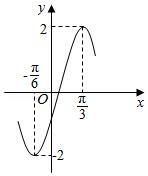
\includegraphics[width=.38\linewidth]{question-3-1.jpg}
\end{center}
\begin{choices}
  \item $y=2\sin(2x-\frac{\pi}{6})$
  \item $y=2\sin(2x-\frac{\pi}{3})$
  \item $y=2\sin(x+\frac{\pi}{6})$
  \item $y=2\sin(x+\frac{\pi}{3})$
\end{choices}
\begin{solution}
\textbf{答案：}$y=2\sin(2x-\frac{\pi}{6})$

\textbf{分析：}由图得$A=2$，$\frac{T}{4}=\frac{\pi}{4}$，故$T=\pi$，$\omega=2$，代入点$(\frac{\pi}{12},2)$得$\varphi=-\frac{\pi}{6}$。
\end{solution}
\end{question}

\begin{question}[points=5]
体积为8的正方体的顶点都在同一球面上，则该球面的表面积为
\begin{choices}
  \item $12\pi$
  \item $\frac{32}{3}\pi$
  \item $8\pi$
  \item $4\pi$
\end{choices}
\begin{solution}
\textbf{答案：}$12\pi$

\textbf{分析：}正方体棱长为2，体对角线为$2\sqrt{3}$，即球直径，半径$\sqrt{3}$，表面积$4\pi(\sqrt{3})^2=12\pi$。
\end{solution}
\end{question}

\begin{question}[points=5]
设$F$为抛物线$C:y^2=4x$的焦点，曲线$y=\frac{k}{x}(k>0)$与$C$交于点$P$，$PF\perp x$轴，则$k=$
\begin{choices}
  \item $\frac{1}{2}$
  \item $1$
  \item $\frac{3}{2}$
  \item $2$
\end{choices}
\begin{solution}
\textbf{答案：}$2$

\textbf{分析：}抛物线焦点$F(1,0)$，由$PF\perp x$轴得$P$横坐标为1，代入$C$得$P(1,2)$，代入$y=\frac{k}{x}$得$k=2$。
\end{solution}
\end{question}

\begin{question}[points=5]
圆$x^2+y^2-2x-8y+13=0$的圆心到直线$ax+y-1=0$的距离为1，则$a=$
\begin{choices}
  \item $-\frac{4}{3}$
  \item $-\frac{3}{4}$
  \item $\sqrt{3}$
  \item $2$
\end{choices}
\begin{solution}
\textbf{答案：}$-\frac{4}{3}$

\textbf{分析：}圆心$(1,4)$，到直线$ax+y-1=0$距离$\frac{|a+4-1|}{\sqrt{a^2+1}}=1$，解得$a=-\frac{4}{3}$。
\end{solution}
\end{question}

\begin{question}[points=5]
如图是由圆柱与圆锥组合而成的几何体的三视图，则该几何体的表面积为
\begin{choices}
  \item $20\pi$
  \item $24\pi$
  \item $28\pi$
  \item $32\pi$
\end{choices}
\begin{solution}
\textbf{答案：}$28\pi$

\textbf{分析：}圆锥母线长$\sqrt{(2\sqrt{3})^2+2^2}=4$，侧面积$\pi\times2\times4=8\pi$；圆柱底面积$\pi\times2^2=4\pi$，侧面积$2\pi\times2\times4=16\pi$，总表面积$28\pi$。
\end{solution}
\end{question}

\begin{question}[points=5]
某路口人行横道的信号灯为红灯和绿灯交替出现，红灯持续时间为40秒。若一名行人来到该路口遇到红灯，则至少需要等待15秒才出现绿灯的概率为
\begin{choices}
  \item $\frac{1}{2}$
  \item $\frac{5}{8}$
  \item $\frac{3}{8}$
  \item $\frac{3}{10}$
\end{choices}
\begin{solution}
\textbf{答案：}$\frac{5}{8}$

\textbf{分析：}红灯持续40秒，至少等15秒，则需在前25秒内到达，概率$\frac{25}{40}=\frac{5}{8}$。
\end{solution}
\end{question}

\begin{question}[points=5]
中国古代有计算多项式值的秦九韶算法，如图是实现该算法的程序框图。执行该程序框图，若输入的$x=2$，$n=2$，依次输入的$a$为2，2，5，则输出的$s=$

\begin{center}
  
\includegraphics[width=.38\linewidth]{question-9-1.jpg}
\end{center}
\begin{choices}
  \item $7$
  \item $12$
  \item $17$
  \item $34$
\end{choices}
\begin{solution}
\textbf{答案：}$17$

\textbf{分析：}模拟：$k=1$，$s=0\times2+2=2$；$k=2$，$s=2\times2+2=6$；$k=3$，$s=6\times2+5=17$，输出$s=17$。
\end{solution}
\end{question}

\begin{question}[points=5]
下列函数中，其定义域和值域分别与函数$y=10^{\lg x}$的定义域和值域相同的是
\begin{choices}
  \item $y=x$
  \item $y=\lg x$
  \item $y=2^x$
  \item $y=\frac{1}{\sqrt{x}}$
\end{choices}
\begin{solution}
\textbf{答案：}$y=\frac{1}{\sqrt{x}}$

\textbf{分析：}$y=10^{\lg x}$定义域和值域均为$(0,+\infty)$。$y=\frac{1}{\sqrt{x}}$定义域和值域均为$(0,+\infty)$，相同。
\end{solution}
\end{question}

\begin{question}[points=5]
函数$f(x)=\cos2x+6\cos(\frac{\pi}{2}-x)$的最大值为
\begin{choices}
  \item $4$
  \item $5$
  \item $6$
  \item $7$
\end{choices}
\begin{solution}
\textbf{答案：}$5$

\textbf{分析：}$f(x)=1-2\sin^2x+6\sin x$，令$t=\sin x\in[-1,1]$，$y=-2t^2+6t+1$，对称轴$t=\frac{3}{2}\notin[-1,1]$，在$[-1,1]$递增，$t=1$时$y_{\max}=5$。
\end{solution}
\end{question}

\begin{question}[points=5]
已知函数$f(x)(x\in\mathbf{R})$满足$f(x)=f(2-x)$，若函数$y=|x^2-2x-3|$与$y=f(x)$图象的交点为$(x_1,y_1)$，$(x_2,y_2)$，…，$(x_m,y_m)$，则$\sum_{i=1}^m x_i=$
\begin{choices}
  \item $0$
  \item $m$
  \item $2m$
  \item $4m$
\end{choices}
\begin{solution}
\textbf{答案：}$m$

\textbf{分析：}函数$f(x)$关于$x=1$对称，$y=|x^2-2x-3|$也关于$x=1$对称，故交点关于$x=1$对称，$\sum x_i = \frac{m}{2}\times2=m$。
\end{solution}
\end{question}

\section*{二、填空题}
本题共4小题，每小题5分。

\begin{question}[points=5]
已知向量$\vec{a}=(m,4)$，$\vec{b}=(3,-2)$，且$\vec{a}\parallel\vec{b}$，则$m=$
\fillin[{$-6$}]
\begin{solution}
\textbf{答案：}$-6$

\textbf{分析：}由向量共线得$m\times(-2)=4\times3$，解得$m=-6$。
\end{solution}
\end{question}

\begin{question}[points=5]
若$x$，$y$满足约束条件$\left\{\begin{array}{l}x-y+1\ge0\\ x+y-3\ge0\\ x\le3\end{array}\right.$，则$z=x-2y$的最小值为

\begin{center}
  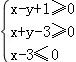
\includegraphics[width=.38\linewidth]{question-14-1.jpg}
\end{center}
\fillin[{$-5$}]
\begin{solution}
\textbf{答案：}$-5$

\textbf{分析：}可行域端点$(3,4)$，代入$z=3-8=-5$最小。
\end{solution}
\end{question}

\begin{question}[points=5]
$\triangle ABC$的内角$A$，$B$，$C$的对边分别为$a$，$b$，$c$，若$\cos A=\frac{4}{5}$，$\cos C=\frac{5}{13}$，$a=1$，则$b=$
\fillin[{$\frac{21}{13}$}]
\begin{solution}
\textbf{答案：}$\frac{21}{13}$

\textbf{分析：}$\sin A=\frac{3}{5}$，$\sin C=\frac{12}{13}$，$\sin B=\sin(A+C)=\frac{63}{65}$，由正弦定理$b=\frac{a\sin B}{\sin A}=\frac{1\times\frac{63}{65}}{\frac{3}{5}}=\frac{21}{13}$。
\end{solution}
\end{question}

\begin{question}[points=5]
有三张卡片，分别写有1和2，1和3，2和3。甲，乙，丙三人各取走一张卡片，甲看了乙的卡片后说：“我与乙的卡片上相同的数字不是2”，乙看了丙的卡片后说：“我与丙的卡片上相同的数字不是1”，丙说：“我的卡片上的数字之和不是5”，则甲的卡片上的数字是
\fillin[{$1$和$3$}]
\begin{solution}
\textbf{答案：}$1$和$3$

\textbf{分析：}推理得甲卡片上的数字是1和3。
\end{solution}
\end{question}

\section*{三、解答题}
解答应写出文字说明、证明过程或演算步骤。

\begin{question}[points=12]
等差数列$\{a_n\}$中，$a_3+a_4=4$，$a_5+a_7=6$。

（Ⅰ）求$\{a_n\}$的通项公式；

（Ⅱ）设$b_n=[a_n]$，求数列$\{b_n\}$的前10项和，其中$[x]$表示不超过$x$的最大整数，如$[0.9]=0$，$[2.6]=2$。
\begin{solution}
\textbf{答案：}（Ⅰ）$a_n=\frac{2n-3}{5}$；（Ⅱ）24

\textbf{分析：}（Ⅰ）设公差$d$，$a_3+a_4=2a_1+5d=4$，$a_5+a_7=2a_1+10d=6$，解得$a_1=\frac{1}{5}$，$d=\frac{2}{5}$，$a_n=\frac{2n-3}{5}$。
（Ⅱ）$b_n=[a_n]$，计算前10项得$b_1=b_2=b_3=1$，$b_4=b_5=2$，$b_6=b_7=b_8=3$，$b_9=b_{10}=4$，和$=3\times1+2\times2+3\times3+2\times4=24$。
\end{solution}
\end{question}

\begin{question}[points=12]
某险种的基本保费为$a$（单位：元），继续购买该险种的投保人称为续保人，续保人本年度的保费与其上年度出险次数的关联如下：



上年度出险次数$\quad0\quad1\quad2\quad3\quad4\quad\ge5$

保费$\quad0.85a\quad a\quad1.25a\quad1.5a\quad1.75a\quad2a$



随机调查了该险种的200名续保人在一年内的出险情况，得到如下统计表：



出险次数$\quad0\quad1\quad2\quad3\quad4\quad\ge5$

频数$\quad60\quad50\quad30\quad30\quad20\quad10$



（Ⅰ）记$A$为事件：“一续保人本年度的保费不高于基本保费”。求$P(A)$的估计值；

（Ⅱ）记$B$为事件：“一续保人本年度的保费高于基本保费但不高于基本保费的160%”。求$P(B)$的估计值；

（Ⅲ）求续保人本年度的平均保费估计值。
\begin{solution}
\textbf{答案：}（Ⅰ）$\frac{11}{20}$；（Ⅱ）$\frac{3}{10}$；（Ⅲ）$1.1925a$

\textbf{分析：}（Ⅰ）保费不高于基本保费的人数$60+50=110$，$P(A)=\frac{110}{200}=\frac{11}{20}$。
（Ⅱ）保费高于基本保费但不高于$1.6a$的人数$30+30=60$，$P(B)=\frac{60}{200}=\frac{3}{10}$。
（Ⅲ）平均保费$=\frac{0.85a\times60+a\times50+1.25a\times30+1.5a\times30+1.75a\times20+2a\times10}{200}=1.1925a$。
\end{solution}
\end{question}

\begin{question}[points=12]
如图，菱形$ABCD$的对角线$AC$与$BD$交于点$O$，点$E$、$F$分别在$AD$，$CD$上，$AE=CF$，$EF$交$BD$于点$H$，将$\triangle DEF$沿$EF$折到$\triangle D'EF$的位置。

（Ⅰ）证明：$AC\perp HD'$；

（Ⅱ）若$AB=5$，$AC=6$，$AE=\frac{5}{4}$，$OD'=2\sqrt{2}$，求五棱锥$D'-ABCFE$体积。

\begin{center}
  
\includegraphics[width=.38\linewidth]{question-19-1.jpg}
\end{center}
\begin{solution}
\textbf{答案：}（Ⅰ）见解析；（Ⅱ）$\frac{9\sqrt{2}}{2}$

\textbf{分析：}（Ⅰ）$AE=CF$得$EF\parallel AC$，且$EF\perp BD$，折后$D'H\perp EF$，故$AC\perp HD'$。
（Ⅱ）$AO=3$，$BO=OD=4$，$DE=\frac{15}{4}$，$EH=\frac{3}{2}$，$EF=3$，$DH=3$，$OH=1$，$OD'=2\sqrt{2}$，$HD'^2=OD'^2+OH^2$，故$OD'\perp$底面，体积$V=\frac{1}{3}\cdot S_{ABCFE}\cdot OD'=\frac{9\sqrt{2}}{2}$。
\end{solution}
\end{question}

\begin{question}[points=12]
已知函数$f(x)=(x+1)\ln x-a(x-1)$。

（Ⅰ）当$a=4$时，求曲线$y=f(x)$在$(1,f(1))$处的切线方程；

（Ⅱ）若当$x\in(1,+\infty)$时，$f(x)>0$，求$a$的取值范围。
\begin{solution}
\textbf{答案：}（Ⅰ）$y=-2x+2$；（Ⅱ）$a\le2$

\textbf{分析：}（Ⅰ）$f(1)=0$，$f'(x)=\ln x+\frac{x+1}{x}-4$，$f'(1)=-2$，切线$y=-2(x-1)=-2x+2$。
（Ⅱ）$f'(x)=1+\frac{1}{x}+\ln x-a$，$f''(x)=\frac{1}{x^2}+\frac{1}{x}>0$，$f'(x)$在$(1,+\infty)$递增，$f'(x)>f'(1)=2-a$。若$a\le2$，$f'(x)\ge0$，$f(x)$递增，$f(x)>f(1)=0$；若$a>2$，存在$x_0$使$f'(x_0)=0$，$f(x)$在$(1,x_0)$递减，$f(x_0)<0$，不合。故$a\le2$。
\end{solution}
\end{question}

\begin{question}[points=12]
已知$A$是椭圆$E:\frac{x^2}{4}+\frac{y^2}{3}=1$的左顶点，斜率为$k(k>0)$的直线交$E$于$A$，$M$两点，点$N$在$E$上，$MA\perp NA$。

（Ⅰ）当$|AM|=|AN|$时，求$\triangle AMN$的面积；

（Ⅱ）当$2|AM|=|AN|$时，证明：$\frac{\sqrt{3}}{3}<k<2$。
\begin{solution}
\textbf{答案：}（Ⅰ）$\frac{144}{49}$；（Ⅱ）见解析

\textbf{分析：}（Ⅰ）$A(-2,0)$，设$M(m-2,m)$，代入椭圆得$7m^2-12m=0$，$m=\frac{12}{7}$，面积$S=m^2=\frac{144}{49}$。
（Ⅱ）$l_{AM}:y=k(x+2)$，$l_{AN}:y=-\frac{1}{k}(x+2)$，联立得$|AM|=\frac{12\sqrt{1+k^2}}{3+4k^2}$，$|AN|=\frac{12\sqrt{1+k^2}}{3k^2+4}$，由$2|AM|=|AN|$得$4k^3-6k^2+3k-8=0$，令$f(k)=4k^3-6k^2+3k-8$，$f'(k)=3(2k-1)^2\ge0$，$f(\frac{\sqrt{3}}{3})<0$，$f(2)>0$，故$\frac{\sqrt{3}}{3}<k<2$。
\end{solution}
\end{question}

\begin{question}[points=10]
如图，在正方形$ABCD$中，$E$，$G$分别在边$DA$，$DC$上（不与端点重合），且$DE=DG$，过$D$点作$DF\perp CE$，垂足为$F$。

（Ⅰ）证明：$B$，$C$，$G$，$F$四点共圆；

（Ⅱ）若$AB=1$，$E$为$DA$的中点，求四边形$BCGF$的面积。

\begin{center}
  
\includegraphics[width=.38\linewidth]{question-22-1.jpg}
\end{center}
\begin{solution}
\textbf{答案：}（Ⅰ）见解析；（Ⅱ）$\frac{1}{2}$

\textbf{分析：}（Ⅰ）$DF\perp CE$得$\triangle DFC\sim\triangle EDC$，$\frac{DF}{CF}=\frac{ED}{DC}$，又$DE=DG$，$CD=BC$，$\angle GDF=\angle BCF$，得$\triangle GDF\sim\triangle BCF$，$\angle GFB=90^\circ$，$\angle GCB=90^\circ$，对角互补，四点共圆。
（Ⅱ）$E$为中点，$AB=1$，$DG=CG=DE=\frac{1}{2}$，$GF=\frac{1}{2}$，$S_{BCGF}=2S_{\triangle BCG}=2\times\frac{1}{2}\times1\times\frac{1}{2}=\frac{1}{2}$。
\end{solution}
\end{question}

\begin{question}[points=10]
在直角坐标系$xOy$中，圆$C$的方程为$(x+6)^2+y^2=25$。

（Ⅰ）以坐标原点为极点，$x$轴正半轴为极轴建立极坐标系，求$C$的极坐标方程；

（Ⅱ）直线$l$的参数方程是$\begin{cases}x=t\cos\alpha\\y=t\sin\alpha\end{cases}$（$t$为参数），$l$与$C$交于$A$，$B$两点，$|AB|=\sqrt{10}$，求$l$的斜率。
\begin{solution}
\textbf{答案：}（Ⅰ）$\rho^2+12\rho\cos\theta+11=0$；（Ⅱ）$\pm\frac{\sqrt{15}}{3}$

\textbf{分析：}（Ⅰ）$x^2+y^2+12x+11=0$，极坐标$\rho^2+12\rho\cos\theta+11=0$。
（Ⅱ）直线$y=\tan\alpha\cdot x$，圆心$C(-6,0)$，半径$5$，弦长$\sqrt{10}$，圆心到直线距离$\frac{|6\tan\alpha|}{\sqrt{1+\tan^2\alpha}}=\frac{3\sqrt{10}}{2}$，解得$\tan^2\alpha=\frac{5}{3}$，$\tan\alpha=\pm\frac{\sqrt{15}}{3}$，斜率$k=\pm\frac{\sqrt{15}}{3}$。
\end{solution}
\end{question}

\begin{question}[points=10]
已知函数$f(x)=|x-\frac{1}{2}|+|x+\frac{1}{2}|$，$M$为不等式$f(x)<2$的解集。

（Ⅰ）求$M$；

（Ⅱ）证明：当$a,b\in M$时，$|a+b|<|1+ab|$。
\begin{solution}
\textbf{答案：}（Ⅰ）$(-1,1)$；（Ⅱ）见解析

\textbf{分析：}（Ⅰ）分类讨论得$f(x)<2$的解为$-1<x<1$，即$M=(-1,1)$。
（Ⅱ）$a,b\in(-1,1)$，则$(a^2-1)(b^2-1)>0$，即$a^2b^2+1>a^2+b^2$，两边加$2ab$得$(ab+1)^2>(a+b)^2$，故$|a+b|<|1+ab|$。
\end{solution}
\end{question}

